\documentclass{article}
\PassOptionsToPackage{quiet}{fontspec}
\usepackage[a4paper, total={6.5in, 10in}]{geometry}
\usepackage{amsmath}
\usepackage{amsfonts}
\usepackage{bm}
% \usepackage{ctex}
\usepackage{tikz}
\usepackage{pgfplots}
\usepgfplotslibrary{patchplots}
\usepgfplotslibrary{fillbetween}
\usepgfplotslibrary{smithchart}
\usepgfplotslibrary{ternary}
\usetikzlibrary{positioning,decorations.markings,arrows.meta, patterns,shapes.arrows}
\usepgfplotslibrary{colorbrewer,colormaps}
\usepgfplotslibrary{polar}
\pgfplotsset{compat=1.17}
\tikzset{
    dot/.style={draw, #1, fill=#1, circle, inner sep=0pt, minimum size=4pt},
    dot/.default={black},
    arrowmark/.style={postaction={decorate, decoration={markings, mark=at position .9 with {\arrow{Stealth}}}}}
}

%% 自定义
\newcommand{\phdi}{\phantom{0}}





\begin{document}
\section{Binomial Tree}

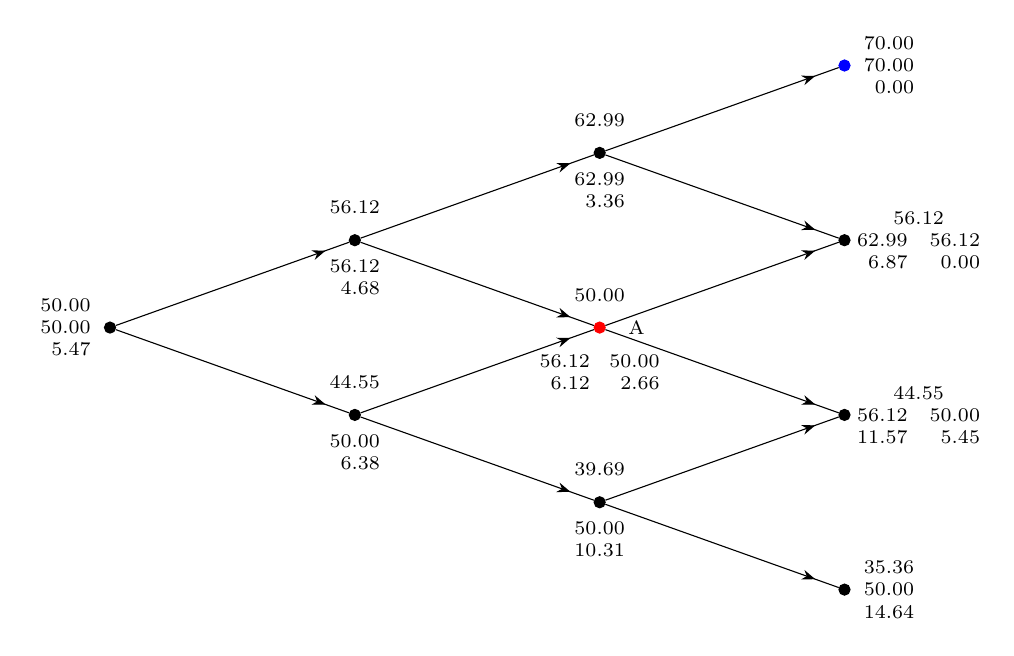
\begin{tikzpicture}[every node/.style={dot}, node distance=1cm and 3cm, align=right, font=\scriptsize]
    \node[label={left:50.00\\50.00\\5.47}](A){};
    \node[above right=of A, label={below:56.12\\4.68}, label={above:56.12}](B1){};
    \node[below right=of A, label={below:50.00\\6.38}, label={above:44.55}](B2){};
    \node[above right=of B1, label={below:62.99\\3.36}, label={above:62.99}](C1){};
    \node[below right=of B1, dot=red, label={[label distance=2.5mm]-120:56.12\\6.12}, label={[label distance=2.5mm]-60:50.00\\2.66}, label={above:50.00}, label={[label distance=2.5mm]right:A}](C2){};
    \node[below right=of B2, label={below:50.00\\10.31}, label={above:39.69}](C3){};
    \node[above right=of C1, dot=blue, label={right:70.00\\70.00\\0.00}](D1){};
    \node[below right=of C1, label={[align=center]right:56.12\\62.99\quad56.12\\\phdi6.87\quad\phdi0.00}](D2){};
    \node[above right=of C3, label={[align=center]right:44.55\\56.12\quad50.00\\11.57\quad\phdi5.45}](D3){};
    \node[below right=of C3, label={right:35.36\\50.00\\14.64}](D4){};
    \draw[arrowmark](A)--(B1); \draw[arrowmark](A)--(B2);
    \draw[arrowmark](B1)--(C1); \draw[arrowmark](B1)--(C2);
    \draw[arrowmark](B2)--(C2); \draw[arrowmark](B2)--(C3);
    \draw[arrowmark](C1)--(D1); \draw[arrowmark](C1)--(D2);
    \draw[arrowmark](C2)--(D2); \draw[arrowmark](C2)--(D3);
    \draw[arrowmark](C3)--(D3); \draw[arrowmark](C3)--(D4);
\end{tikzpicture}


\section{ColorMap}

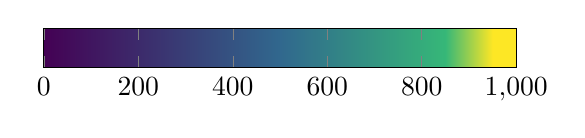
\begin{tikzpicture}
\pgfplotscolorbardrawstandalone[
    colormap={example}{
        of colormap={
            viridis,
            target pos={0,500,850,950,1000},
            sample for=const,
        },
    },
    colorbar horizontal,
    colormap access=map
    ]
\end{tikzpicture}
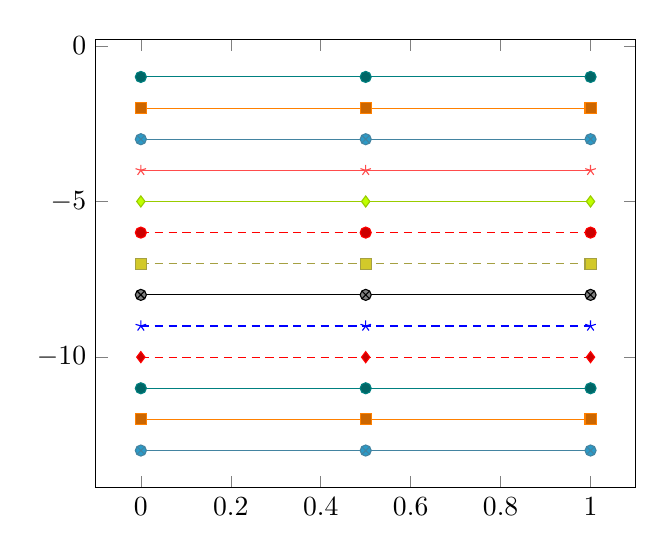
\begin{tikzpicture}
    \begin{axis}[
        stack plots=y,stack dir=minus,
        cycle list name=exotic,
    ]
    \addplot coordinates {(0,1) (0.5,1) (1,1)};
    \addplot coordinates {(0,1) (0.5,1) (1,1)};
    \addplot coordinates {(0,1) (0.5,1) (1,1)};
    \addplot coordinates {(0,1) (0.5,1) (1,1)};
    \addplot coordinates {(0,1) (0.5,1) (1,1)};
    \addplot coordinates {(0,1) (0.5,1) (1,1)};
    \addplot coordinates {(0,1) (0.5,1) (1,1)};
    \addplot coordinates {(0,1) (0.5,1) (1,1)};
    \addplot coordinates {(0,1) (0.5,1) (1,1)};
    \addplot coordinates {(0,1) (0.5,1) (1,1)};
    \addplot coordinates {(0,1) (0.5,1) (1,1)};
    \addplot coordinates {(0,1) (0.5,1) (1,1)};
    \addplot coordinates {(0,1) (0.5,1) (1,1)};
    \end{axis}
\end{tikzpicture}

\section{Function Plot}

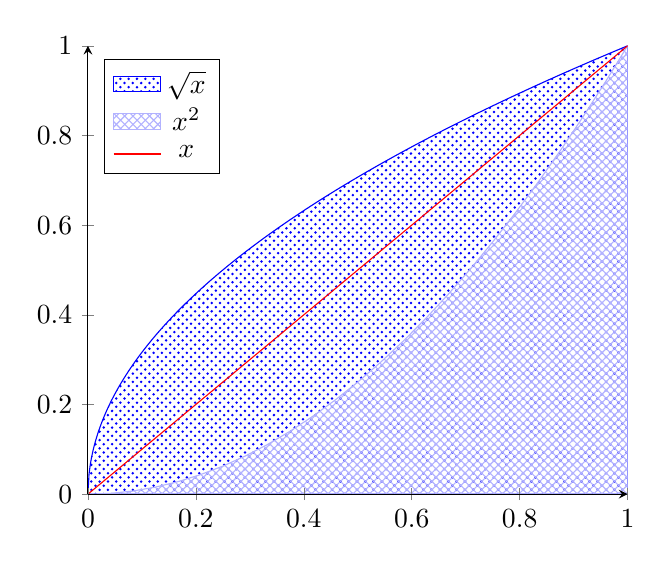
\begin{tikzpicture}
    \begin{axis}[area legend,
    axis x line=bottom,axis y line=left,
    domain=0:1,
    legend pos=north west,
    axis on top,xmin=0,
    ]
    \addplot [pattern=crosshatch dots,
    pattern color=blue,draw=blue,
    samples=500]
    {sqrt(x)} \closedcycle;
    \addplot [pattern=crosshatch,
    pattern color=blue!30!white,
    draw=blue!30!white]
    {x^2} \closedcycle;
    \addplot [red,line legend]
    coordinates {(0,0) (1,1)};
    \legend{$\sqrt x$,$x^2$,$x$}
    \end{axis}
\end{tikzpicture}
\begin{tikzpicture}
    \begin{axis}[
    minor tick num=3,
    axis y line=left,
    axis x line=middle,
    xlabel=$x$,ylabel=$\sin x$,
    ]
    \addplot [
    smooth,blue,mark=none,
    domain=-5:5,samples=40,
    ] {sin(deg(x))};
    \end{axis}
\end{tikzpicture}

\section{Colormap with Function}
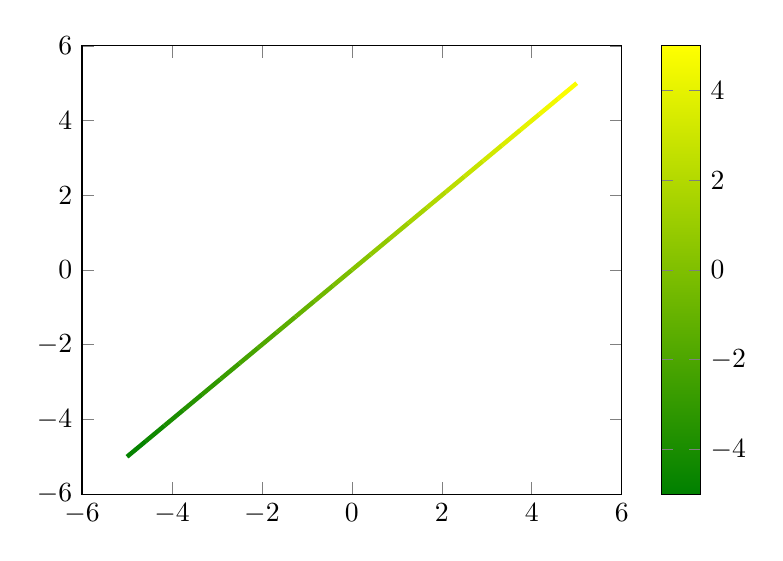
\begin{tikzpicture}
    \begin{axis}[colorbar,colormap/greenyellow]
    \addplot [mesh,ultra thick] {x};
    \end{axis}
\end{tikzpicture}
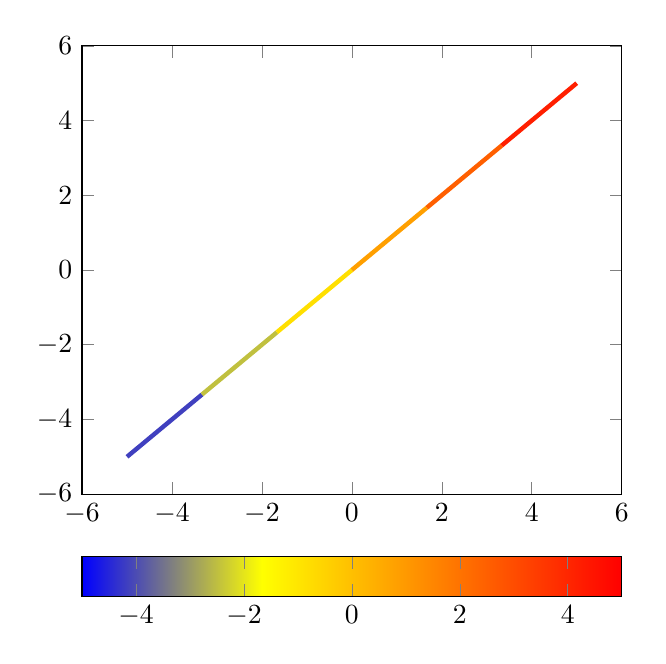
\begin{tikzpicture}
    \begin{axis}[colorbar horizontal]
    \addplot [mesh,ultra thick,samples=7] {x};
    \end{axis}
\end{tikzpicture}



\section{Scatter Plot}
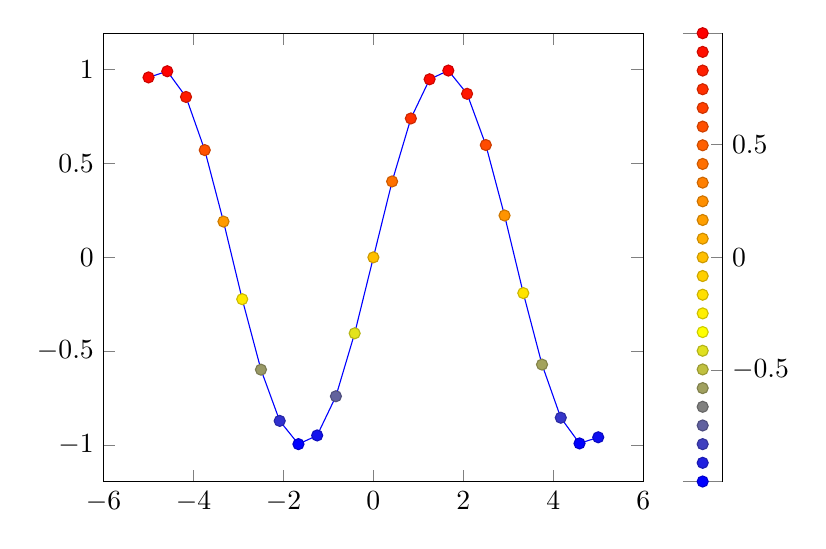
\begin{tikzpicture}
    \begin{axis}[colorbar sampled line]
    \addplot+ [scatter] {sin(deg(x))};
    \end{axis}
\end{tikzpicture}
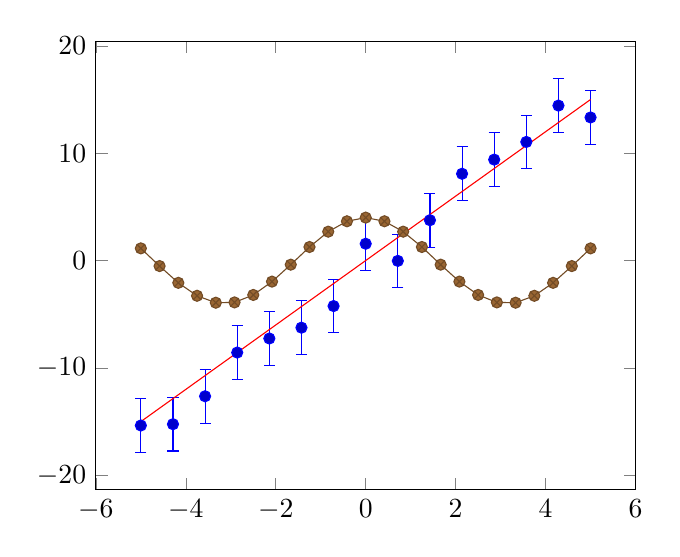
\begin{tikzpicture}[baseline]
    \begin{axis}
    \addplot+ [
    only marks,
    samples=15,
    error bars/y dir=both,
    error bars/y fixed=2.5,
    ] {3*x+2.5*rand};
    \label{pgfplots:label1}
    \addplot+ [mark=none] {3*x};
    \label{pgfplots:label2}
    \addplot {4*cos(deg(x))};
    \label{pgfplots:label3}
    \end{axis}
\end{tikzpicture}

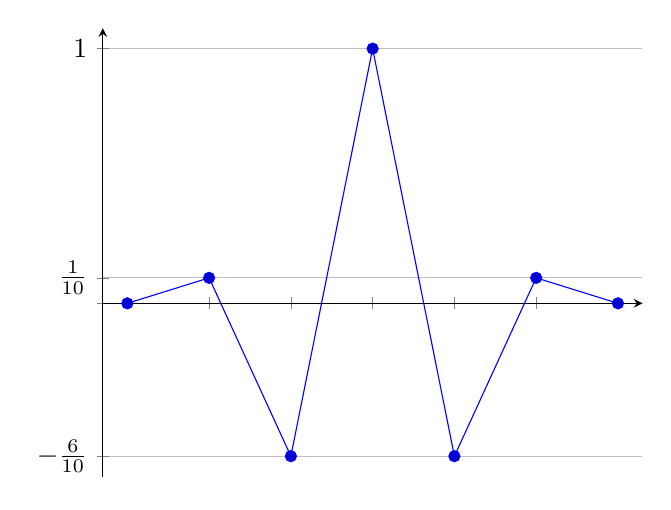
\begin{tikzpicture}
    \begin{axis}[
    xtick=data,
    axis x line=center,
    xticklabels={,,},
    ytick={-0.6,0,0.1,1},
    yticklabels={
    $-\frac{6}{10}$,,
    $\frac{1}{10}$,$1$},
    ymajorgrids,
    axis y line=left,
    enlargelimits=0.05
    ]
    \addplot coordinates {
    (-3,0) (-2,0.1) (-1,-0.6)
    (0,1)
    (1,-0.6) (2,0.1) (3,0)
    };
    \end{axis}
\end{tikzpicture}
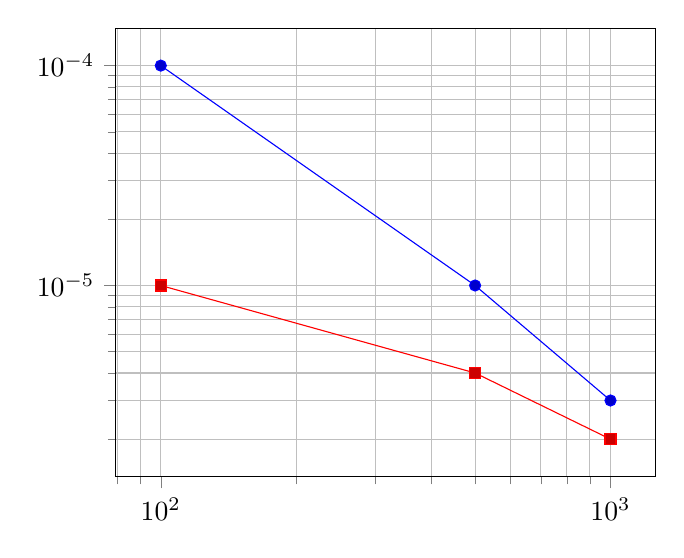
\begin{tikzpicture}
    \begin{loglogaxis}[
    grid=both,
    tick align=outside,
    tickpos=left,
    ]
    \addplot coordinates {
    (100,1e-4) (500,1e-5) (1000,3e-6)
    };
    \addplot coordinates {
    (100,1e-5) (500,4e-6) (1000,2e-6)
    };
    \end{loglogaxis}
\end{tikzpicture}


\section{ParamPlot}
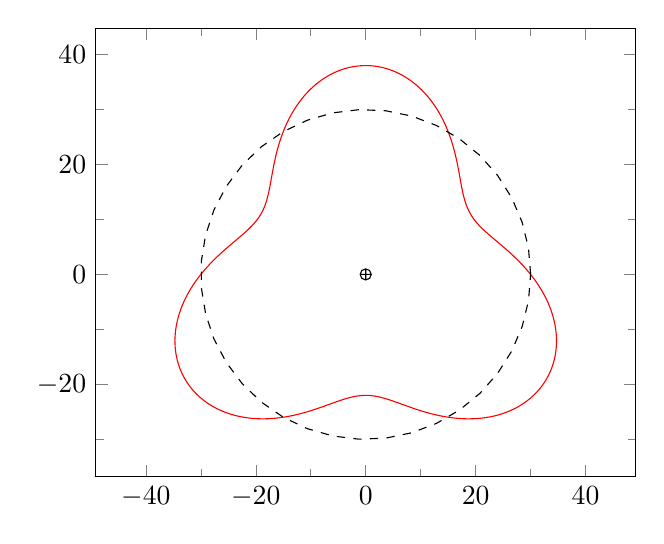
\begin{tikzpicture}
    \begin{axis}[
    axis equal,
    minor tick num=1,
    ]
    \def\FREQUENCY{3}
    \addplot [red,domain=0:360,samples=200,
    smooth,data cs=polar]
    (x,{30-8*sin(\FREQUENCY*x)});
    \addplot [samples=40,domain=0:2*pi,dashed,
    data cs=polar] (deg(x),30);
    \addplot [mark=oplus,only marks] coordinates {(0,0)};
    \end{axis}
\end{tikzpicture}
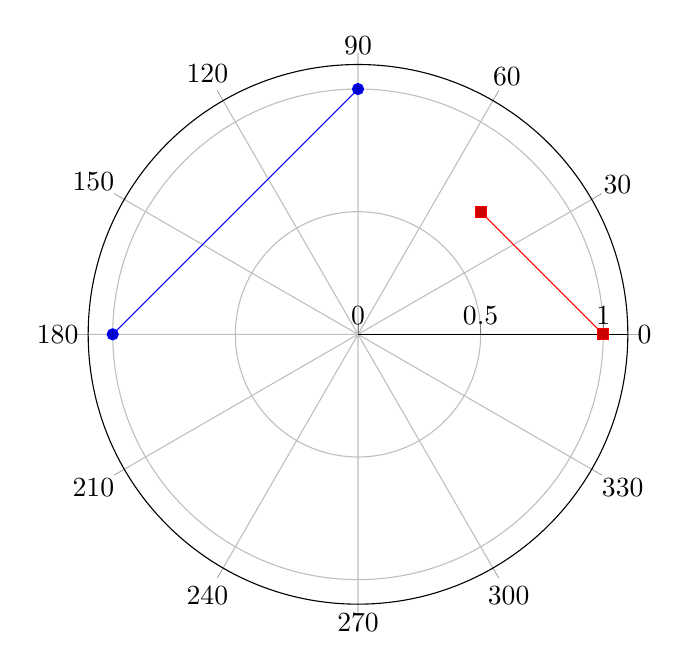
\begin{tikzpicture}
    \begin{polaraxis}
    \addplot coordinates {(90,1) (180,1)};
    \addplot+ [data cs=cart] coordinates {
    (1,0)
    (0.5,0.5)
    };
    \end{polaraxis}
\end{tikzpicture}



\section{Matri Grid Distri}
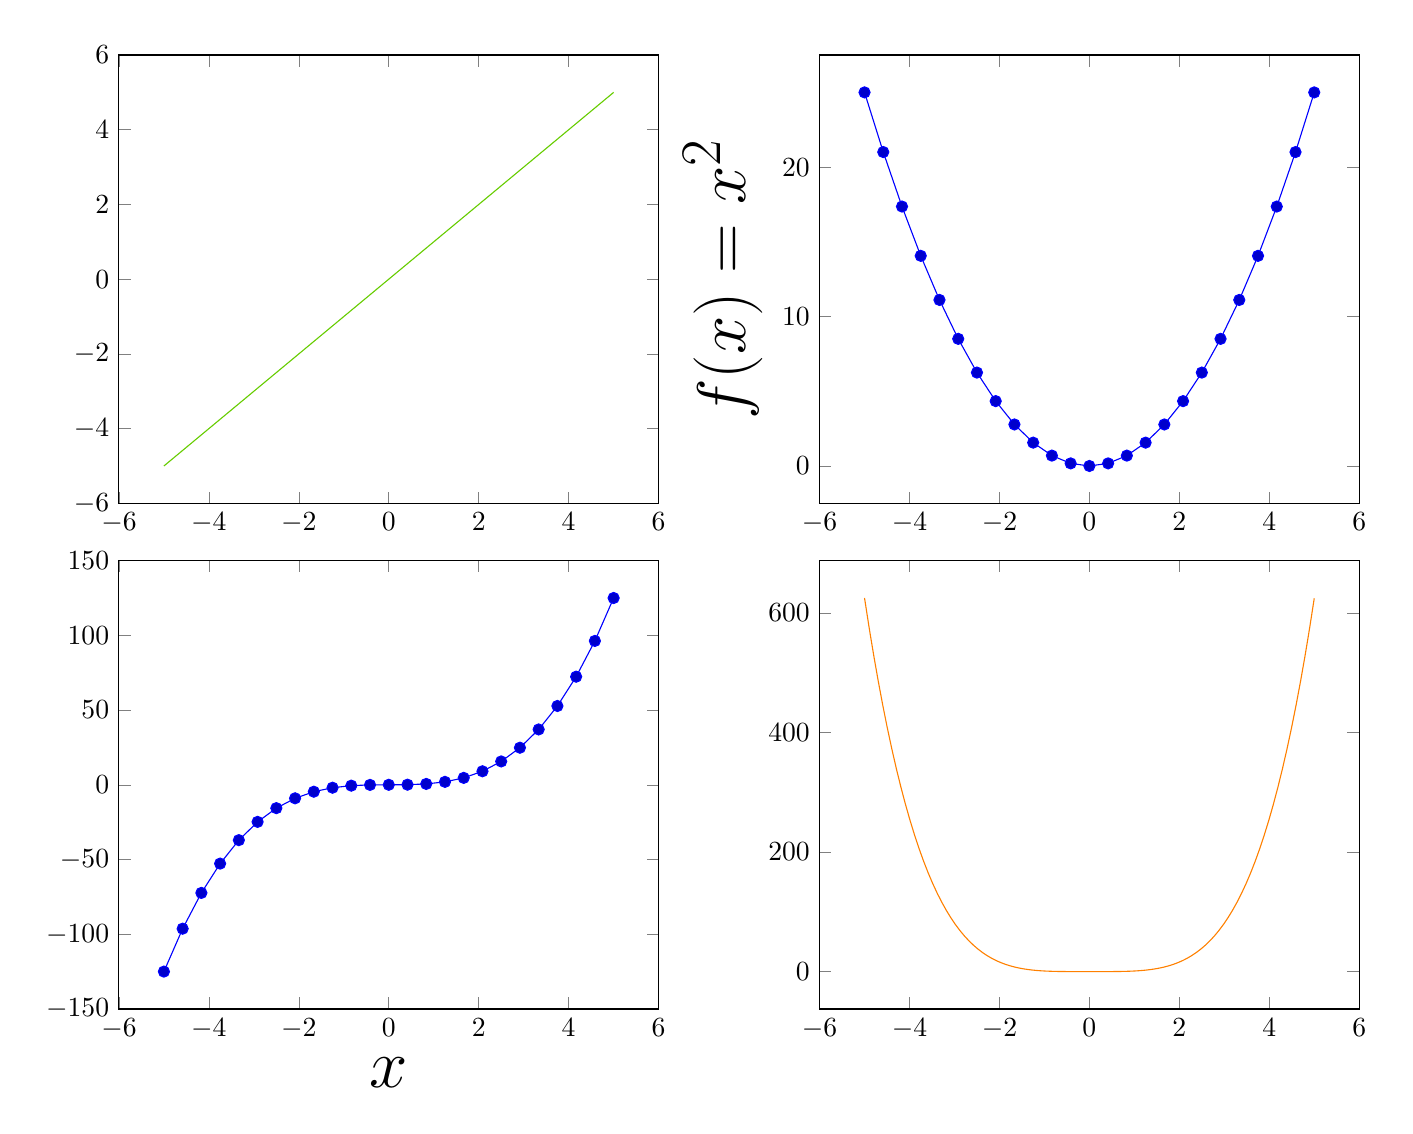
\begin{tikzpicture}
    \matrix {
            \begin{axis}
            \addplot[draw=orange!40!green] {x};
            \end{axis}
            &
            % differently large labels are aligned automatically:
            \begin{axis}[ylabel={$f(x)=x^2$},ylabel style={font=\Huge}]
            \addplot {x^2};
            \end{axis}
        \\
            \begin{axis}[xlabel=$x$,xlabel style={font=\Huge}]
            \addplot {x^3};
            \end{axis}
            &
            \begin{axis}
            \addplot[draw=orange,samples=100] {x^4};
            \end{axis}
        \\
    };
\end{tikzpicture}

\section{Varible Scatter}
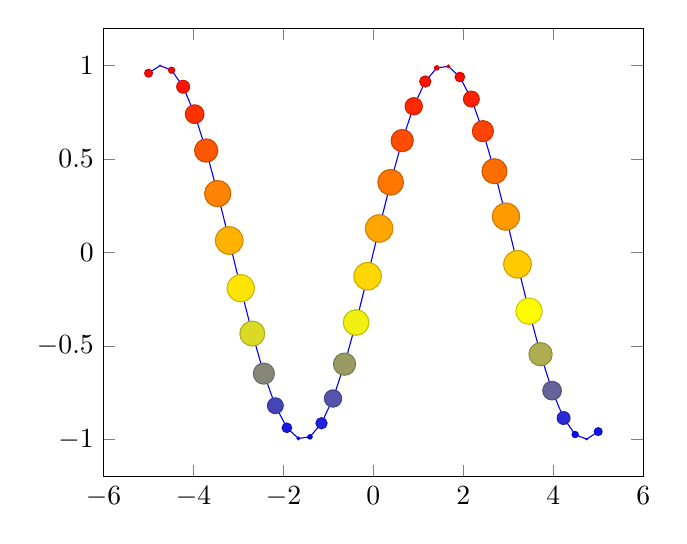
\begin{tikzpicture}
    \begin{axis}
    \addplot+ [
    scatter,
    scatter src=y,
    samples=40,
    visualization depends on=
    {5*cos(deg(x)) \as \perpointmarksize},
    scatter/@pre marker code/.append style=
    {/tikz/mark size=\perpointmarksize},
    ]
    {sin(deg(x))};
    \end{axis}
\end{tikzpicture}
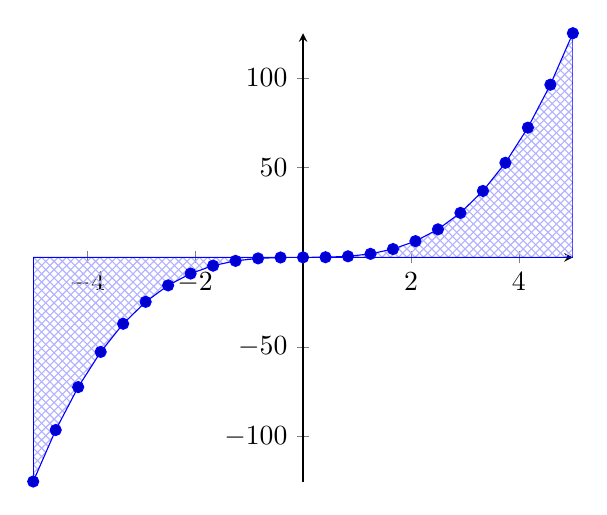
\begin{tikzpicture}
    \begin{axis}[
    axis on top=false,
    axis x line=middle,
    axis y line=middle,
    ]
    \addplot+[pattern=crosshatch,pattern color=blue!30!white] {x^3} \closedcycle;
    \end{axis}
\end{tikzpicture}


\section{Filling}
\;\lower-10em\hbox{An Complex Example }
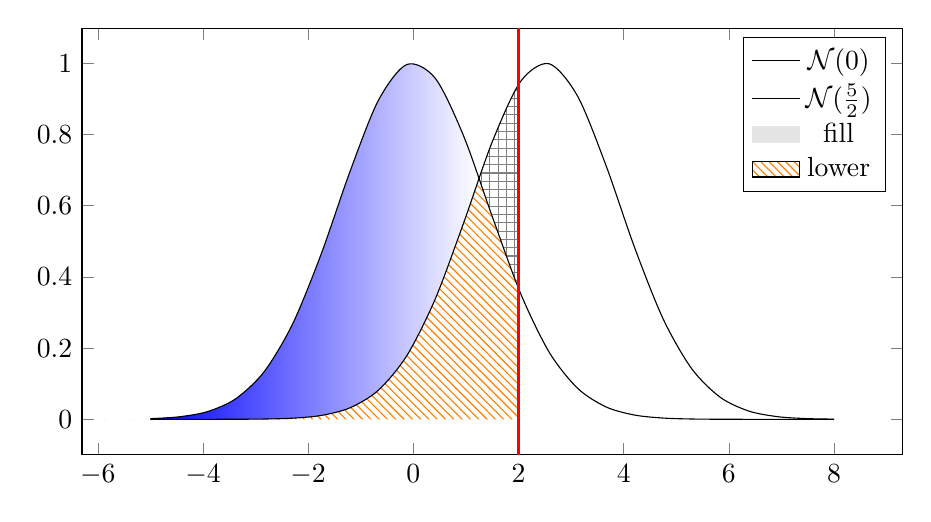
\begin{tikzpicture}
    \def\verticalbar{2}
    \begin{axis}[domain=-5:8,samples=25,smooth,width=12cm,height=7cm]
        % Draw curves
        \addplot [name path=g0,thin] {exp(-x^2/4)};
        \addlegendentry{$\mathcal{N}(0)$}
        \addplot [name path=g2.5,thin] {exp(-(x-2.5)^2/4)};
        \addlegendentry{$\mathcal{N}(\frac52)$}
        % Draw vertical bar:
        \draw [name path=red,red,thick](\verticalbar,-1) -- (\verticalbar,2);
        \path [name path=axis] (-10,0) -- (16,0);
        \addplot [black!10] fill between [
            of=g0 and g2.5,
            soft clip={domain=-6:\verticalbar},
            split,
            every segment no 0/.style={left color=blue,right color=white},
            every segment no 1/.style={pattern=grid,pattern color=gray},
        ];
        \addlegendentry{fill}
        % compute + label the lower segment (but do not draw it):
        \path [name path=lower,
            %draw=red,ultra thick,
            intersection segments={of=g0 and g2.5,sequence=R1 -- L2}
        ];
        \addplot [pattern=north west lines, pattern color=orange]
            fill between [
            of=axis and lower,
            soft clip={domain=-6:\verticalbar},
        ];
        \addlegendentry{lower}
    \end{axis}
\end{tikzpicture}

\subsection{Filling an Area}
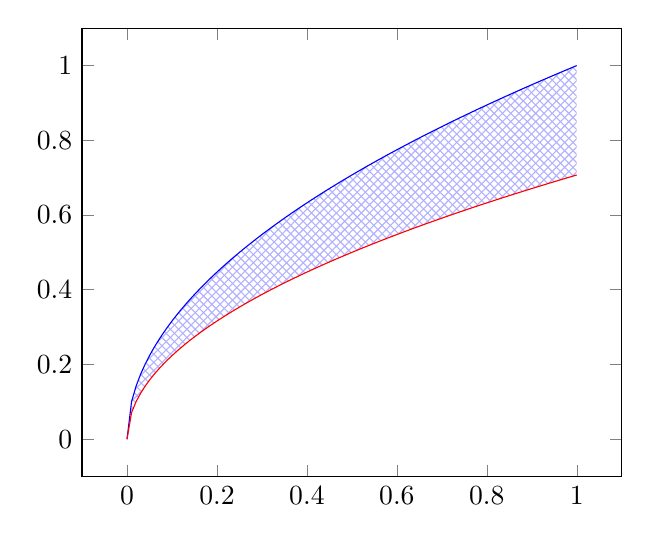
\begin{tikzpicture}
    \begin{axis}
    \addplot [blue,name path=A,domain=0:1,samples=100] {sqrt(x)};
    \addplot [red, name path=B,domain=0:1,samples=100] {sqrt(x/2)};
    \addplot [pattern=crosshatch,pattern color=blue!30!white] fill between [of=A and B];
    \end{axis}
\end{tikzpicture}
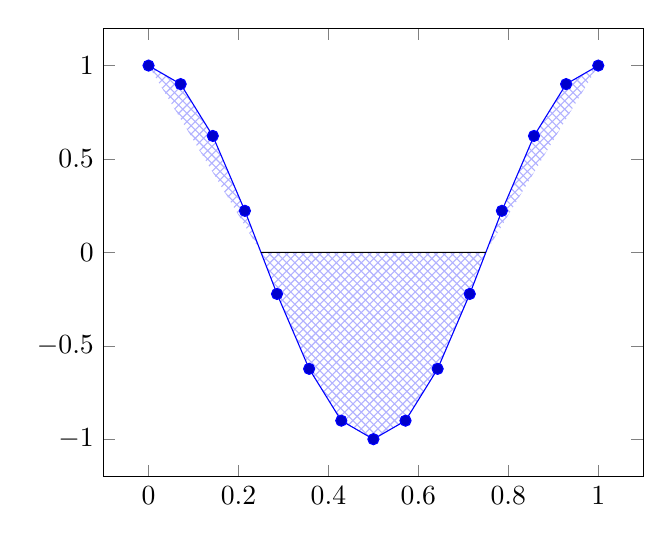
\begin{tikzpicture}
    \begin{axis}
        \addplot+ [name path=A,samples=15,domain=0:1]{cos(360*x)}
                coordinate [pos=0.25] (nodeA0) {}
                coordinate [pos=0.75] (nodeA1) {};
        \draw [name path=B](nodeA0) -- (nodeA1);
        \addplot [pattern=crosshatch,pattern color=blue!30!white] fill between [of=A and B];
    \end{axis}
\end{tikzpicture}

\subsection{Filling Different Segments of the Area}
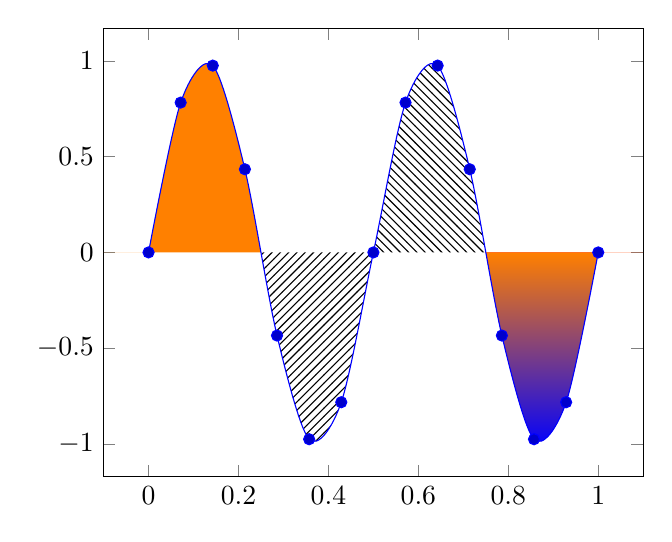
\begin{tikzpicture}
    \begin{axis}
        \addplot+ [name path=A,samples=15,smooth,domain=0:1] {sin(720*x)};
        \path [name path=B](\pgfkeysvalueof{/pgfplots/xmin},0) -- (\pgfkeysvalueof{/pgfplots/xmax},0);
        \addplot fill between [of=A and B, split,every segment no 0/.style=
            {orange},
            every segment no 1/.style=
            {pattern=north east lines},
            every segment no 2/.style=
            {pattern=north west lines},
            every segment no 3/.style=
            {top color=orange, bottom color=blue},
        ];
    \end{axis}
\end{tikzpicture}
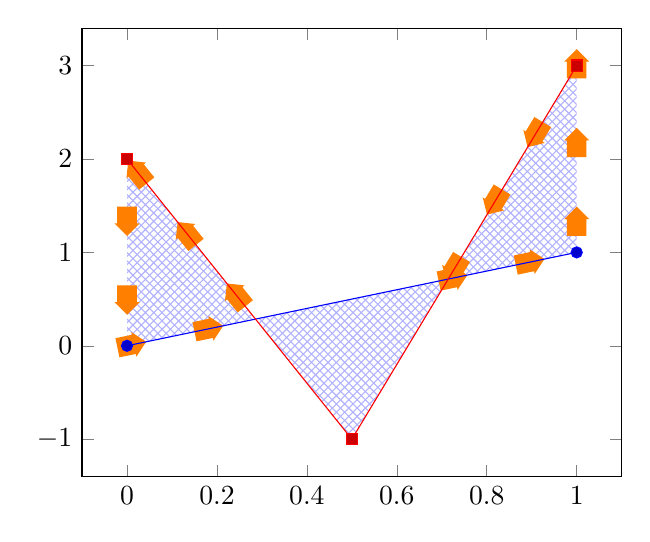
\begin{tikzpicture}
    \begin{axis}
        \addplot+ [name path=A,domain=0:1,samples=2] {x};
        \addplot+ [name path=B] table {
            x y
            0 2
            0.5 -1
            1 3
        };
        \addplot[pattern=crosshatch,pattern color=blue!30!white] fill between [of=A and B,split,
            every even segment/.style={
            postaction={decorate},
            decoration={
                markings,
                mark=between positions 0 and 1
                step 1cm with {
                    \node [single arrow,fill=orange,
                    single arrow head extend=1pt,
                    transform shape]
                    {};
                },
            },
        },];
    \end{axis}
\end{tikzpicture}

\subsection{Clip Filling}
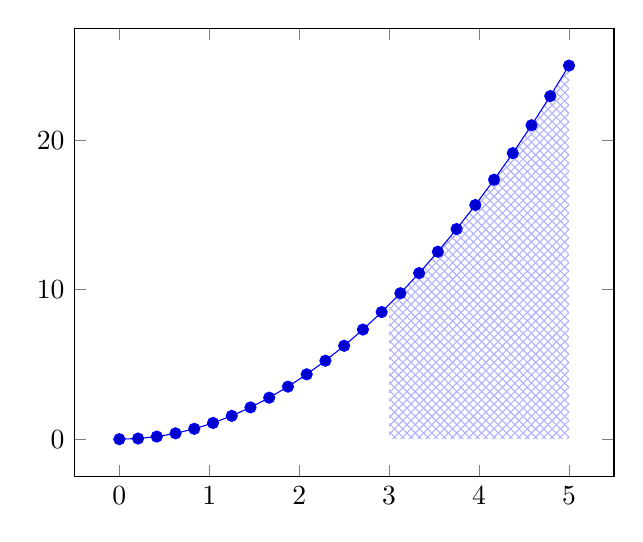
\begin{tikzpicture}
    \begin{axis}
        \addplot+ [name path=A,domain=0:5] {x^2};
        \path [name path=B]
            (\pgfkeysvalueof{/pgfplots/xmin},0) --
            (\pgfkeysvalueof{/pgfplots/xmax},0);
        \addplot [pattern=crosshatch,pattern color=blue!30!white] fill between [
            of=A and B,
            soft clip={domain=3:5},
        ];
    \end{axis}
\end{tikzpicture}
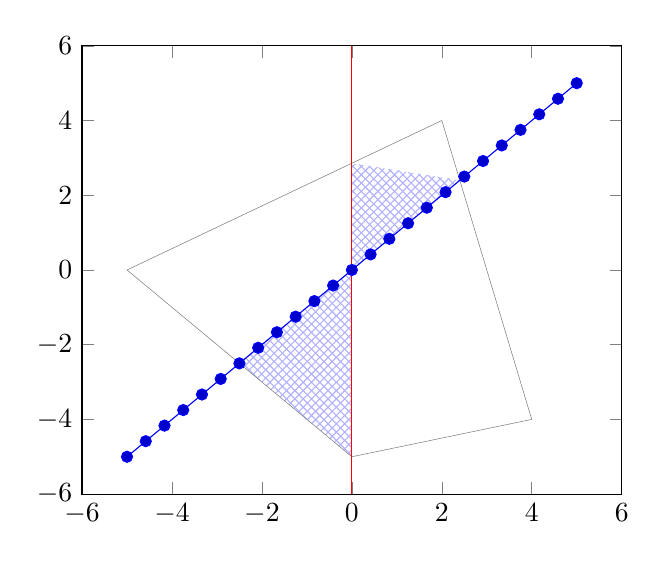
\begin{tikzpicture}
    \begin{axis}
        \draw [help lines,name path=clippath]
            (0,-5) -- (-5,0) --
            (2,4) -- (4,-4) --cycle;
        \addplot+ [name path=A] {x};
        \draw [red,name path=B]
            (0,\pgfkeysvalueof{/pgfplots/ymin}) --
            (0,\pgfkeysvalueof{/pgfplots/ymax});
        \addplot[pattern=crosshatch,pattern color=blue!30!white] fill between [
            of=A and B,
            soft clip={clippath}
        ];
    \end{axis}
\end{tikzpicture}

\subsection{Key Reference}
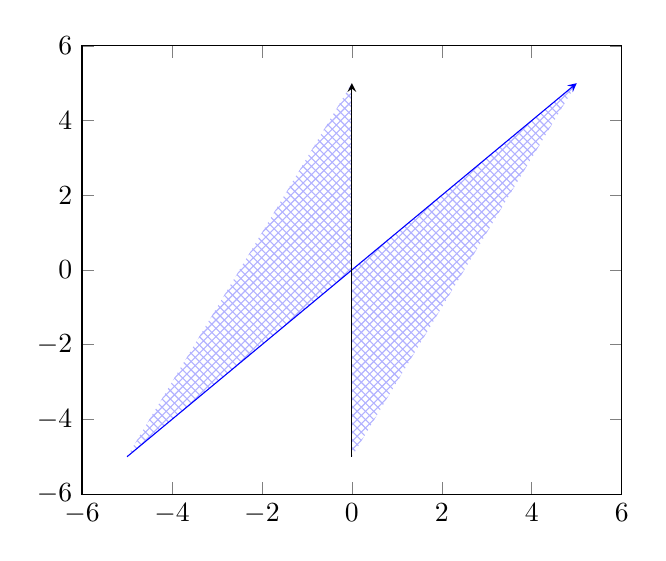
\begin{tikzpicture}
    \begin{axis}[set layers]
        \addplot [blue,-stealth,name path=A] {x};
        \draw [-stealth,name path=B]
            (0,-5) -- (0,5);
        \pgfonlayer{pre main}
        \fill [
            pattern=crosshatch,pattern color=blue!30!white,
            intersection segments={
                of=A and B,
                sequence={A* -- B*},
            },
        ];
        \endpgfonlayer
    \end{axis}
\end{tikzpicture}
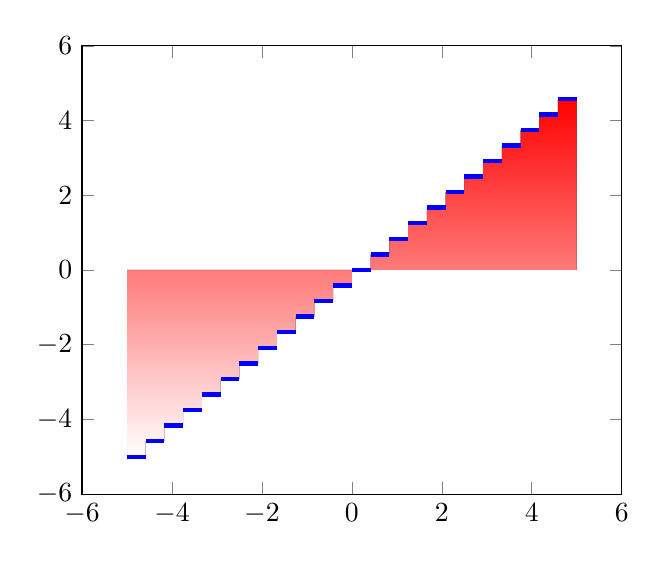
\begin{tikzpicture}
    \begin{axis}
        \addplot [blue,ultra thick,name path=A,
            jump mark left] {x};
        \path [name path=B]
            (-5,0) -- (5,0);
        \addplot [top color=red, bottom color=white]
            fill between [of=A and B];
    \end{axis}
\end{tikzpicture}


\section{3D Scatter}
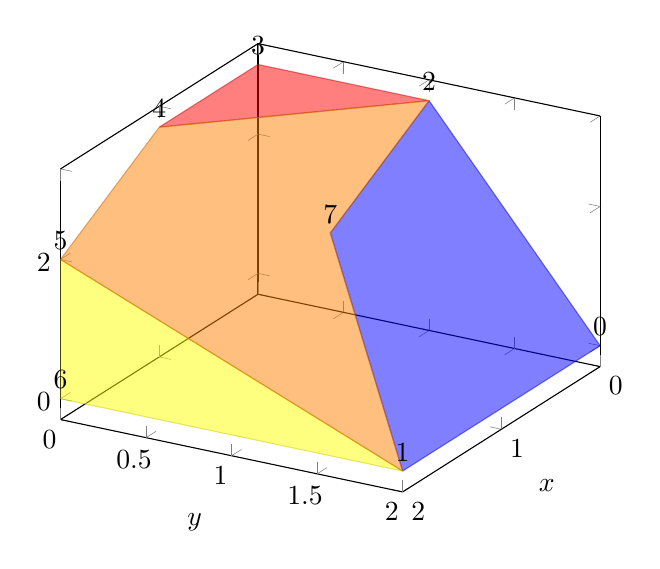
\begin{tikzpicture}
    \begin{axis}[view/h=120,xlabel=$x$,ylabel=$y$]
        \addplot3 [
            opacity=0.5,
            table/row sep=\\,
            patch,
            patch type=polygon,
            vertex count=5,
            patch table with point meta={
            % pt1 pt2 pt3 pt4 pt5 cdata
            0 1 7 2 2 0\\
            1 6 5 5 5 1\\
            1 5 4 2 7 2\\
            2 4 3 3 3 3\\
        },
        ] table {
            x y z\\
            0 2 0\\%0
            2 2 0\\%1
            0 1 3\\%2
            0 0 3\\%3
            1 0 3\\%4
            2 0 2\\%5
            2 0 0\\%6
            1 1 2\\%7
        };
        % replicate the vertex list to show \coordindex:
        \addplot3 [only marks,nodes near coords=\coordindex,] 
        table [row sep=\\] {
            0 2 0\\ 2 2 0\\ 0 1 3\\ 0 0 3\\
            1 0 3\\ 2 0 2\\ 2 0 0\\ 1 1 2\\
        };
    \end{axis}
\end{tikzpicture}
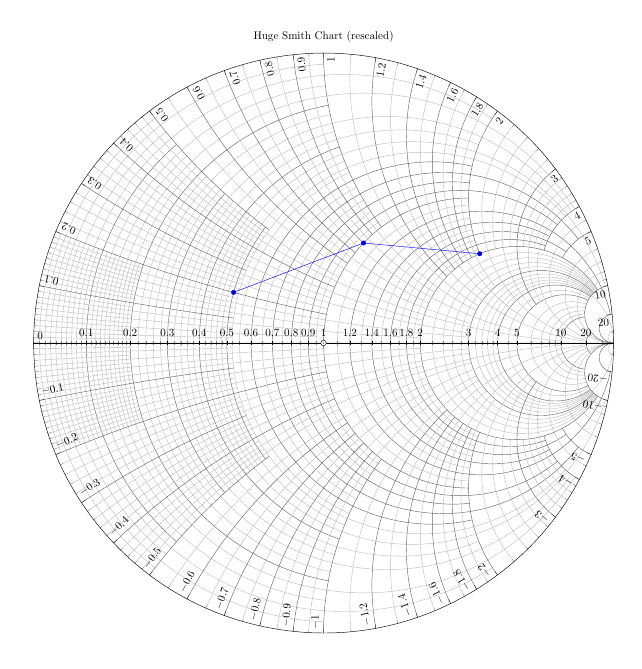
\begin{tikzpicture}[scale=0.4]
    \begin{smithchart}[
        title=Huge Smith Chart (rescaled),
        width=20cm,
    ]
    \addplot coordinates {(0.5,0.2) (1,0.8) (2,2)};
    \end{smithchart}
\end{tikzpicture}

\section{Ternary}
\noindent
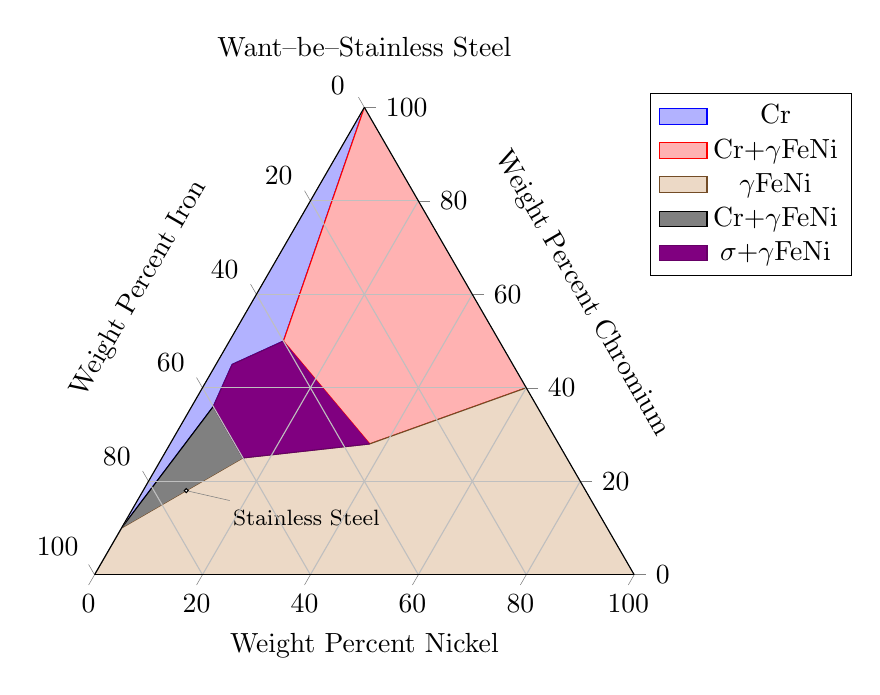
\begin{tikzpicture}
    \begin{ternaryaxis}[
        title=Want--be--Stainless Steel,
        xlabel=Weight Percent Chromium,
        ylabel=Weight Percent Iron,
        zlabel=Weight Percent Nickel,
        label style=sloped,
        area style,
    ]
    \addplot3 table {
        A B C
        1 0 0
        0.5 0.4 0.1
        0.45 0.52 0.03
        0.36 0.6 0.04
        0.1 0.9 0
    };
    \addlegendentry{Cr}
    \addplot3 table {
        A B C
        1 0 0
        0.5 0.4 0.1
        0.28 0.35 0.37
        0.4 0 0.6
    };
    \addlegendentry{Cr+$\gamma$FeNi}
    \addplot3 table {
        0.4 0 0.6
        0.28 0.35 0.37
        0.25 0.6 0.15
        0.1 0.9 0
        0 1 0
        0 0 1
    };
    \addlegendentry{$\gamma$FeNi}
    \addplot3 table {
        0.1 0.9 0
        0.36 0.6 0.04
        0.25 0.6 0.15
    };
    \addlegendentry{Cr+$\gamma$FeNi}
    \addplot3 table {
        0.5 0.4 0.1
        0.45 0.52 0.03
        0.36 0.6 0.04
        0.25 0.6 0.15
        0.28 0.35 0.37
    };
    \addlegendentry{$\sigma$+$\gamma$FeNi}
    \node [
        inner sep=0.5pt,
        circle,draw,fill=white,
        pin=-15:\footnotesize Stainless Steel
    ]
    at (0.18,0.74,0.08) {};
    \end{ternaryaxis}
\end{tikzpicture}
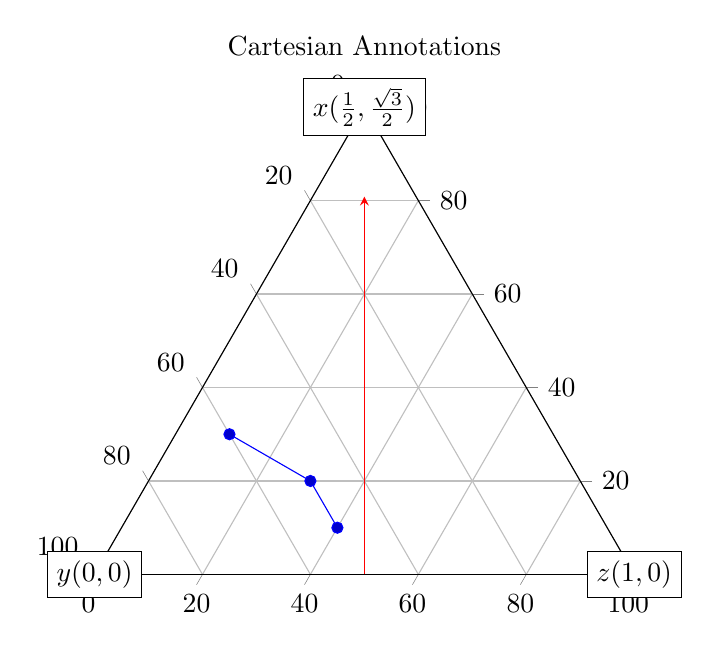
\begin{tikzpicture}
    \begin{ternaryaxis}[
            title=Cartesian Annotations,
            clip=false,
        ]
        \addplot3 coordinates {
            (0.1,0.5,0.4)
            (0.2,0.5,0.3)
            (0.3,0.6,0.1)
        };
        \node [fill=white,draw]
            at (cartesian cs:0,0) {$y (0,0)$};
        \node [fill=white,draw]
            at (cartesian cs:1,0) {$z (1,0)$};
        \node [fill=white,draw]
            at (cartesian cs:0.5,{sqrt(3)/2})
            {$x (\frac12,\frac{\sqrt3}{2})$};
        \draw [red,-stealth]
            (cartesian cs:0.5,0)-- (cartesian cs:0.5,0.7);
    \end{ternaryaxis}
\end{tikzpicture}









\end{document}
































